\documentclass[12pt]{report}
\usepackage{fontspec}
\usepackage{polyglossia}
\usepackage{amsthm}
\usepackage{amsmath}
\usepackage{amssymb}
\usepackage{esint}
\usepackage[left=30mm, top=20mm, right=30mm, bottom=20mm, nohead, nofoot]{geometry}

\newtheorem{definition}{Определение}
\newtheorem{theorem}{Теорема}
\newtheorem{lemma}{Лемма}
\newtheorem{example}{Пример}

\setdefaultlanguage{russian}
\setmainfont[Mapping=tex-text]{CMU Serif}

\begin{document}

\section{Определения и обозначения}

$\Omega \in \mathbb{R}, \Omega$ - область

$L^1(\Omega), \quad L^p(\Omega) := \{ u: \: \int_{\Omega}|u(x)|^pdx < + \infty\}$

$L^\infty(\Omega) := \{ u: \exists c > 0, |u(x)| \le c \: a.e. x \}$

$\mathfrak{F} = F(x), x \in \mathbb{R}, x = (x_1, ..., x_n)$

Обозначения частной производной: 
$$
    \frac{\partial f}{\partial x_r}, \quad \partial_{x_r}f, \quad \partial_rf, \quad f_{x_r}, \quad f,x_r, \quad f, _r
$$

Ни в коем случае не писать так: 
$$
    \frac{df}{dx_r}
$$

$\partial \Omega$ - топологическая граница, $\overline{\Omega}$ - замыкание


\chapter{Классическая теория уравнений в частных производных}

\section{Распространение пятна загрязнения в канале}

Представим, что в канал попала загрязняющая жидкость. Перед нами стоит задача поиска закона,
по которому будет распространяться пятно загрязнения в данном канале. 
Как это можно расписать? 

Для начала, будем считать, что пятно -- одномерная зона. $v$ - скорость течения воды в канале. 

Пусть у нас есть момент времени $t \in \mathbb{R^+}$. В точке $x \in \mathbb{R}$ в момент времени $t = 0$ концентрация загрязняющего вещества в воде будет представлена функцией $c_0(x) = c(0, x)$, где $c(t,x)$ - концентрация вещества в момент $t$.

Можем воспользоваться законом сохранения массы
$$
    \int^{x + \Delta x}_{x}{c(t, \xi)d\xi}
$$

$q(t,x)$ -- поток массы вещества в момент $t$ по направлению от точки $x$ вправо.

$$\frac{d}{dt} \int^{x + \Delta x}_{x}{c(t, \xi)d\xi} = -q(t, x + \Delta x) + q(t, x)$$

Считаем, что можно пронести производную под знак интеграла, т.е. функция q(t,x) гладкая, существуют непрерывные производные. Тогда: 
$$
    \fint_{x}^{x + \Delta x}{c_t(t, \xi)d\xi} = \frac{q(t,x) - q(t, x+ \Delta x)}{\Delta x}
$$

Интервал $\Delta x$ может быть сколь угодно мал. Т.к. все функции здесь гладкие, можно перейди к пределу: 

\begin{equation} \label {law:diff}
    c_t(t, x) = - q_x(t,x)    
\end{equation}

    -- Дифференциальный Закон


Как устроен поток? От чего он может зависеть? Рассмотрим три случая:
\begin{itemize}
    \item Диффузия
    \item Конвекция
    \item И то, и другое
\end{itemize}

\subsection{Диффузия}

Предположим, что загрязняющее вещество хорошо диффузирует, вода стоячая, т.е. $v=0$. Тогда масса распространяется броуновским движением от того места, где концентрация вещества больше, до того, где ее меньше. 
Т.е, поток зависит от концентрации.

$$q(t,x) = Kc_x(t,x) = -Dc_x(t,x),$$
где $K$ -- коэффициент, зависящий от среды, $D$ -- коэффициент диффузии

Подставим закон в \eqref{law:diff} и получим: 

\begin{equation} \label{eq:diffusion}
    c_t(t,x) = Dc_xx(t,x)
\end{equation}
    -- Уравнение Диффузии (или Уравнение Теплопроводности)
    
(Это уравнение означает, что в момент времени $t$ поток через стенку $x$ пропорционален градиенту концентрации)
    
Например, пусть речь идет об одномерной ложке. Распределение тепла вдоль длины ложки описывается тем же законом.

\subsection{Конвекция}
Пусть диффузии нет. Чистая конвекция. Тогда поток есть просто $q(t,x) = vc(t,x)$.
Подставим это в \eqref{law:diff} и получим: 
$$c_t(t,x) = -vc_x(t,x)$$

или 

\begin{equation} \label{eq:transport}
    c_t(t,x) + vc_x(t,x) = 0
\end{equation}
-- Транспортное Уравнение (или Уравнение Переноса)

Заметим, что уравнение \eqref{eq:diffusion} -- линейное уравнение частных производных 2-ого порядка, а уравнение \eqref{eq:transport} -- линейное уравнение в частных производных 1-ого порядка. 

\subsection{Диффузия и конвекция}

Если на поток влияют оба явления, получаем, что: 
$$q(t,x) = -Dc_x(t,x) + vc_x(t,x)$$

Подставим данное уравнение в \eqref{law:diff}: 
$$c_t(t,x) = Dc_xx(t,x) - vc_x(t,x)$$

\begin{equation} \label{eq:Fokker-Planck}
    c_t + vc_x = Dc_xx
\end{equation}
    -- Уравнение Фоккера-Планка
    
\section{Решение однородного транспортного уравнения}

Имеем задачу: 
\begin{equation} \label{pro:Cauchy}
    \begin{cases}
        c_t + vc_x = 0
        \\
        c(0,x) = c_0(x)
    \end{cases}
\end{equation}

    -- Задача Коши (начальная задача) для транспортного уравнения. 
    
Решений первого уравнения системы очень много, но нас интересует конкретное. Для этого берем условие -- второе уравнение системы.

Как решить задачу Коши? К тому, что в данном случае значит "решить" подойдем интуитивно. Функция должна быть гладкой, производные непрерывными (поточечно и там, где решение существует). Таким образом, получаем Классическое Решение. Ни о каких других решениях пока ничего не знаем. 

Рассматриваем всё ту же задачу о распространении пятна загрязнения в канале. Масса этого пятна состоит из частиц. Каждая частица этой массы эволюционирует по закону: 
$$x(0) = x_0, \quad x(t) = x_0 + vt$$

\begin{equation}
    \begin{cases}
        \frac{dx}{dt} = v
        \\
        x \vert_{t=0} = x_0
    \end{cases}
\end{equation}
    
Пусть c(t,x) - решение транспортного уравнения. Как это решение ведет себя вдоль интегральной кривой? 
    
Представим ситуацию: человек сидит на одной из частиц нашего пятна загрязнения. Если он посмотрит вокруг себя, то ничего не заметит. Вокруг него ничего не меняется. 
    
Предположим, что $c(t,x(t))$ -- константа. Для того, чтобы проверить эту догадку, продифференцируем $c(t,x(t))$ (производная должна быть равна 0):
    
$$\frac{d}{dt}c(t,x(t)) = c_t(t,x(t)) + c_x(t,x(t))\frac{dx}{dt} = c_t + vc_x = 0$$
    
Т.е вдоль траектории ОДУ концентрация не меняется. Что получилось? Вдоль каждой прямой (луча) концентрация постоянна. Каждой прямой соответствует частица. И нет таких точек, через которые бы не проходила ни одно интегральная кривая (из простоты дифференциального уравнения)
    
\begin{equation} 
    c(t,x) = c_0(x-vt)    
\end{equation}
    
$$
    \begin{gathered}
        x = x_0 + vt \Longrightarrow x_0 = x - vt
        \\
        c(0, x - vt) = c_0(x - vt)
    \end{gathered}
$$

\begin{definition}
    Обыкновенное дифференциальное уравнение, вдоль траектории которого решения уравнения в частных производных постоянны, называется характеристическим. 
\end{definition}

\begin{definition}
    Траектории характеристического уравнения называются характеристическими линиями (или характеристиками)
\end{definition}

Решение вдоль характеристик постоянно. Оказалось, что решение существует единственно и всюду. Мы нашли формулу для решения задачи Коши, подставив начальное значение.

Проверим, что выполняются условия \eqref{pro:Cauchy}. Для этого сформулируем теорему.

\begin{theorem}
    Если $c_0 \in C^1(\mathbb{R})$, то \eqref{pro:Cauchy} имеет единственное классическое решение в виде $c(t,x) = c_0(x-vt)$.
\end{theorem}

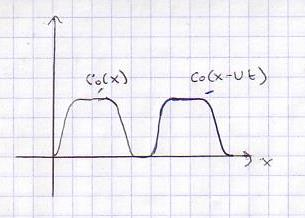
\includegraphics{wave.jpg}

В начальный момент времени $t = 0$ имеем контур. После, сдвигаем направо на $vt$. Получаем "бегущую волну". То есть, профиль нашего загрязнения при увеличении $t$ смещается по течению.

Для того, чтобы функция была классическим решением, она должна быть гладкой. Но даже если это не так, в физике подобная функция будет считаться решением задачи, если такое решение будет физически осмысленно. 

\section{Решение неоднородного транспортного уравнения}

Имеем задачу:
\begin{equation} \label{pro:CauchyInhom}
    \begin{cases}
        c_t + vc_x = f(t,x)
        \\
        c(0, x) = c_0(x)
    \end{cases}
\end{equation}

-- Задача Коши для неоднородного транспортного уравнения. 

В этом случа предполагается, что загрязнение поступило не единовременно, а существует некоторый источник загрязнения. 
Тогда $f(t,x)$ -- есть мощность источника загрязнения. 

$$\frac{d}{dt}c(t, x(t)) = c_t + c_x \frac{dx}{dt} = c_t + vc_x = f(t, x(t))$$

$$\forall x_0: \quad \frac{d}{dt}c(t, x_0 - vt) = f(t, x_0 + vt)$$

$$c(t, x_0 + vt) = c(0,x_0) + \int^{0}_{t}{f(s, x_0 + vs)ds}$$

$$x_0 + vt = x \Longrightarrow x_0 = x - vt$$

$$c(t,x) = c(0, x - vt) + \int^{0}_{t}{f(s, x - vt + vs)ds} \Longrightarrow $$

\begin{equation} \label{eq:solutionInhom}
    c(t, x) = c_0(x - vt) + \int^{0}_{t}{f(s, x - v(t - s))ds}
\end{equation}

Таким образом, получили формулу для решения, теперь надо понять, когда оно существует и единственно ли?

$$ \bigl ( \int^{0}_{t}{f(s, x - v(t-s))ds} \bigr )_t = f(t, x) - v \int^{0}_{t}{f_x(s, x - v(t - s))ds}$$

$$ \bigl ( \int^{0}_{t}{f(s, x - v(t-s))ds} \bigr )_x = \int^{0}_{t}{f_x(s, x - v(t - s))ds}$$

\begin{theorem}
    Если $c_0 \in C^1(\mathbb{R}), \; f \in C(\mathbb{R} ^ + \times \mathbb{R}), \: f_x \in C(\mathbb{R} ^ + \times \mathbb{R})$, то существует единственное решение задачи \eqref{eq:solutionInhom} и оно имеет вид \eqref{pro:CauchyInhom}.
\end{theorem}

Пояснение: единственность следует из того, что если $c$ -- решение, то оно обязано быть в таком виде. Иначе, пусть решений два: 
$c_1$ и $c_2$, $c = c_1 - c_2$
$$c_t + vc_x = (c_1 - c_2)_t + v(c_1 - c_2)_x = ((c_1)_t + v(c_1)_x) - ((c_2)_t + v(c_2)_x) = 0 \Longrightarrow c_1 = c_2$$

\section{Основная лемма вариационного исчисления}

\begin{lemma}[Слабый вариант]
    $\Omega \subset \mathbb{R} ^ n$ -- область, $f \in C(\Omega):$
    $$\int_{\Omega}{f(x)g(x)dx} = 0 \quad \forall \: g \in C_0 ^\infty (\Omega) $$
    Тогда $f \equiv 0$
\end{lemma}

\begin{definition}
    Носителем функции $g$ называется 
    $$supp(g) := \overline{\{x: \: g(x) \ne 0 \}}$$
\end{definition}

\begin{example}
    $\Omega \subset \mathbb{R}$; $\Omega = (-1, 1)$
    
    $v(x) = 1 - x^2, v(x) \in C^\infty (\Omega)$
    
    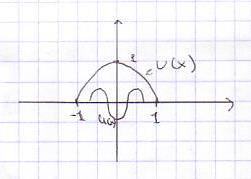
\includegraphics{compfunc.jpg}
    
    У $v(x)$ нет компактного носителя, т.к. он не находится строго внутри $\Omega$.
\end{example}

\begin{lemma}[Сильная формулировка]
    $\Omega \subseteq \mathbb{R} ^ n$ -- область
    
    $f \in L_{loc}(\Omega)$ (т.е. $f$ локально суммируема на $\Omega$)
    
    $$\int_{\Omega}{f(x)g(x)dx} = 0 \quad \forall \: g \in C_0^\infty(\Omega)$$
    
    Тогда $f = 0$ почти везде в $\Omega$
\end{lemma}

\begin{example}
    $e^x$ -- интегрируема на $\mathbb{R}$? Нет. Но на компакте -- да, т.е. она интегрируема локально. 
    
    Напомним:
    
    Почти всюду в $\Omega \Longleftrightarrow e = \{x: \: f(x) = 0 \}, \; \mu(e) = 0$
\end{example}

\begin{proof}[Доказательство (леммы со слабой формулировкой)]
    От противного: 
    
    Пусть $f \in C(\Omega)$ и $\exists x_0 \in \Omega \colon \; f(x_0) > 0$ $\Longrightarrow \exists r>0 \colon f(x) > 0 \; \forall x \in B_r(x_0)$ (т.к. $f \in C(\Omega)$) $B_r(x_0) \subset \Omega$
    
    Возьмем $g \in C^\infty(\Omega) \colon $
    
    $$
        \begin{cases}
            g(x) > 0 & \forall x \in B_r(x_0)
            \\
            g(x) = 0 & \forall x \in B_r^c(x_0) = \Omega  B_r(x_0)
        \end{cases}
    $$
    
    $$supp(g) = \overline{B_r(x_0) \subseteq \Omega} \Longrightarrow g \in C_0^\infty(\Omega)$$
    
    По условию имеем, что $\int_{\Omega}{f(x)g(x)dx} = 0$.
    
    Внутри $B_r(x_0) \colon \; f(x), g(x) > 0$. Следовательно, и $\int_{\Omega}{f(x)g(x)dx} > 0$. Откуда приходим к противоречию. Тогда $f \equiv 0$
    
    Осталось доказать существование такой функции $g$. 
    
    Построим её: 
    $$\psi \colon \mathbb{R} \longrightarrow \mathbb{R}; \quad 
        \psi(x) = 
        \begin{cases}
            e^{\frac{1}{x^2 - 1}} & x \in (-1, 1)
            \\
            0 & x \notin (-1, 1)
        \end{cases}
    $$
    
    Нужно доказать, что $e^{\frac{1}{x^2 - 1}} \in C^\infty (-1, 1)$.
    
    $g(x) := \psi(\frac{|x-x_0|}{r})$
    
\end{proof}
    
\section{Колебание струны и волновое уравнение}
Имеется струна. Ей придают начальную скорость и дергают, выводя из состояния равновесия. "Движущаяся, растягивающаяся, сжимающаяся пружина". Струна, относительно положения равновесия, смещается по закону $u = u(t,x)$, где $t$ -- время, $x$ -- координата вдоль струны.

\subsection{Вывод уравнения колебания струны}

Как описать динамику механической системы? $T$ -- кинетическая энергия, $U$ -- потенциальная энергия. Тогда
$$A = \int^{\theta}_{0}{(T-U)dt}$$

Наш интерес представляет задача $$A = \int^{\theta}_{0}{(T-U)dt} \longrightarrow \min$$

Зафиксируем кусочек струны длиной $L$. Если $\Delta x$ очень маленькое, какая будет скорость? 

$u_t$ -- скорость. Кусочек струны имеет небольшую массу. Можно взять плотность -- $\rho_0$, и умножить ее на длину этого кусочка. Тогда кинетическая энергия в момент t будет равна: 

$$T = \int^{L}_{0}{\rho_0 \frac{u_t^2}{2}dx}$$

Как найти потенциальную энергию? До колебания длина элемента так и была $\Delta x$. С колебанием она стала длиной други. Длина дуги равна $$\int_{x}^{x + \Delta x}{\sqrt{1 + u_x^2}dx}$$.

Тогда растяжение или сжатие струны вычисляется так: 
$$\int_{x}^{x + \Delta x}{\sqrt{1 + u_x^2}dx} - \Delta x = \int_{x}^{x + \Delta x}{(\sqrt{1 + u_x^2} - 1)dx} \approx $$

Так как $\Delta x$ (т.е. смещение) очень мало, воспользуемся формулой Тейлора:

$$ \approx \int_{x}^{x + \Delta x}{(1 + \frac{1}{2}u_x^2 - 1)dx} = \frac{1}{2}u_x^2 \Delta x$$

Тогда по всей струне

$$U(x) \approx \int_{0}^{L}{\tau_0 \frac{u_x^2}{2}dx}$$

где $\tau_0$ -- начальное натяжение, определяемое жесткостью струны. 

Тогда
$$A = \int_{0}^{\tau}{dt} \bigl ( \int_{0}^{L}{\frac{\rho_0}{2}u_t^2dx} - \int_{0}^{L}{\frac{\tau_0}{2}u_x^2dx} \bigr ) = $$

$$ \frac{1}{2} \int^{\tau}_{0}{dt \int^{L}_{0}{(\rho_0 u_t^2 - \tau_0 u_x^2)dx}} \longrightarrow min$$

$$A(u) = \frac{1}{2} \int^{\tau}_{0}{dt \int^{L}_{0}{(\rho_0 u_t^2 - \tau_0 u_x^2)dx}}$$

Пусть нашли такое $u$, что $A(u)$ минимально. 

$v \in C_0^\infty((0, L) \times (0, \tau))$

$A(u + \epsilon v) \ge A(u)$ -- следует из минимальности $u$

$A(u = \epsilon v) - A(u) \ge 0$

$$
    \begin{cases}
        \frac{A(u + \epsilon v) - A(u)}{\epsilon} \ge 0 & \epsilon > 0
        \\
        \frac{A(u + \epsilon v) - A(u)}{\epsilon} \le 0 & \epsilon < 0
    \end{cases}
$$

Перейдем к пределу:

$$
    \lim_{\epsilon \longrightarrow 0}{\frac{A(u + \epsilon v) - A(u)}{\epsilon}} = A'(u)v = \frac{d}{d \epsilon}A(u + \epsilon v) \vert_{\epsilon = 0}
$$

$$
    \begin{cases}
        \frac{A(u + \epsilon v) - A(u)}{\epsilon} \longrightarrow A'(u)v \ge 0 & \epsilon > 0
        \\
        \frac{A(u + \epsilon v) - A(u)}{\epsilon} \longrightarrow A'(u)v \le 0 & \epsilon < 0
    \end{cases}
$$

$$
    A'(u)v = 0
$$
-- если такая производная осмыслена. 

Получили первую вариацию точки $u$ по направлению $v$. 

\begin{definition}
    Пусть $F$ -- функционал, определенный на области $\Omega$ и $v \in C_0^\infty(\Omega)$. Тогда функционал 
    $$
        F'(u)v = \lim_{\epsilon \longrightarrow 0}{\frac{F(u + \epsilon v) - F(u)}{\epsilon}}
    $$
    называется производной $F$ в точке $u$ по направлению $v$.
\end{definition}

$$
    \begin{cases}
        A'(u)v \ge 0 & \epsilon > 0
        \\
        A'(u)v \le 0 & \epsilon < 0
    \end{cases}
$$

Проверим, что первую вариацию можно получить. При этом считаем, что все функции гладкие, производные непрерывны и ограничены. Можем пронести производную под знак интеграла: 
$$
    \begin{gathered}
        A'(u)v = \frac{d}{d \epsilon}A(u + \epsilon v) \vert_{\epsilon = 0} = \frac{d}{d \epsilon}\int^{\tau}_{0}{dt \int^{L}_{0}{dx(\rho_0 \frac{(u_t + \epsilon v_t) ^ 2}{2} - \tau_0 \frac{(u_x+ \epsilon v_x) ^ 2}{2}) \vert_{\epsilon = 0}}} =
        \\
        = \int^{\tau}_{0}{dt \int^{L}_{0}{dx (\rho_0 \frac{2}{2}(u_t + \epsilon v_t)v_t - \tau_0 \frac{2}{2}(u_x + \epsilon v_x)v_x) \vert_{\epsilon = 0}}} = 
        \\
        = \int^{\tau}_{0}{dt \int^{L}_{0}{dx (\rho_0 u_t v_t - \tau_0 u_x v_x)}}
    \end{gathered}
$$

Таким образом, доказали, что производная существует, просто ее посчитав. 

Так как мы старались минимизировать $A$, получаем, что такой интеграл должем быть равен нулю. При этом хотим избавиться от производных $v_x$ и $v_t$.

Проинтегрируем по частям: 

$$
\begin{gathered}
    = - \int^{\tau}_{0}{dt \int^{L}_{0}{dx(\rho_0 u_{tt} v - \tau_o u_{xx}v)}} =
    \\
    = - \int^{\tau}_{0}{dt \int^{L}_{0}{dx v (u_{tt}\rho_0 - \tau_0 u_{xx})}} = 0 
\end{gathered}
$$

Напоминает основную лемму вариационного исчисления.
$$
    \int_{0}^{\tau}{dt \int^{L}_{0}{dx(u_{tt} \rho_0 - \tau_0 u_{xx})}} = 0
$$

А это возможно тогда, когда $\rho_0 u_{tt} - \tau_0 u_{xx} = 0$ всюду на $(0, \tau) \times (0, L)$.
$$u_{tt} - \frac{\tau_0}{\rho_0}u_{xx} = 0$$Обозначим $c^2 := \frac{\tau_0}{\rho_0}$.

Получили 

\begin{equation} \label{eq:wave}
    u_{tt} - c ^ 2 u_{xx} = 0
\end{equation}

-- Волновое уравнение. 

Заметим, что оно является уравнением в частных производных 2-ого порядка. Также обратим внимание на то, что $\tau$ мы могли взять из $(0, +\infty)$, как и $L$. Следовательно, \eqref{eq:wave} верно на $(0, +\infty) \times (0, +\infty)$.

Волновое уравнение описывает колебание струны. А что было бы, будь на месте струны мембрана? Что бы изменилось в таком случае? 

Действие тоже было бы интегралом от кинетической и потенциальной энергии. $u = u(t,x,y)$. Интеграл был бы по $\Omega$.

Для вычисления потенциальной энергии брали бы элемент площади. 
$$
    u_x^2 + u_y^2 = (u_x, u_y) \bullet (u_x, u_y)
$$
-- пространственный градиент. Произведение здесь скалярное. 

$\bigtriangledown u \bullet \bigtriangledown u = |\bigtriangledown u| ^ 2$

Уравнение имело бы вид: 
$$u_{tt} - c ^ 2(u_{xx} + u_{yy}) = 0$$

$$u_{xx} + u_{yy} = div(u_x, u_y)$$

Что такое дивергенция? 

$\mathbb{R}$ -- скалярное поле. $u = u(x_1, ..., x_n)$.

$$
    \begin{gathered}
        grad \; u = \bigtriangledown u = ( \frac{\partial u}{\partial x_1, ..., \frac{\partial u}{\partial x_n}})
        \\
        F: \mathbb{R} ^ n \longrightarrow \mathbb{R} ^ n, \: F = (F_1(x), ..., F_n(x))
        \\
        div \; F = \bigtriangledown \bullet F = \frac{\partial F_1}{\partial x_1} + ... + \frac{\partial F_n}{\partial x_n}
    \end{gathered}
$$

В частности, если $u = u(x, y)$, то $grad \; u = \bigtriangledown u = (u_x, u_y)$

$$
    \begin{gathered}
        div \; \bigtriangledown u = \bigtriangledown \bullet \bigtriangledown u = u_{xx} + u_{yy} = \bigtriangleup u
        \\
        \bigtriangledown = (\frac{\partial}{\partial x_1}, ..., \frac{\partial}{\partial x_n})
        \\
        u = u(x, y, z) \quad \bigtriangledown u = (u_x, u_y, u_z)
        \\
        div \bigtriangledown u = \bigtriangledown \bigtriangledown u = (u_{xx} u_{yy} + u_{zz}) = \bigtriangleup u
    \end{gathered}
$$

Все производные только по пространственным переменным (мы в физике).

$$
    \begin{gathered}
        u_{tt} - c^2 (u_{xx} + u_{yy}) = 0
        \\
        u_{tt} - c ^ 2 \bigtriangleup u = 0 \; \text{в} \; \mathbb{R} ^ + \times \Omega 
    \end{gathered}
$$
Так как $\bigtriangleup u = u_{xx} + u_{yy}$. А для волны звука измерений было бы три. 

Таким образом, получаем общий случай Волнового Уравнения: 

\begin{equation} \label{eq:gen_wave}
    u_{tt} - c ^ 2 \bigtriangleup u = 0 
\end{equation}

$\Box_c u = u_{tt} - c ^ 2 \bigtriangleup u = 0$ -- оператор Д'Аламбера

$\Box_{c ^ 2} = 0$ -- обозначение волнового уравнения.

Какие задачи здесь можно ставить и решать? 

\section{Задача о колебании бесконечной струны}

Чем более точную имеем модель, тем сложнее получить решение. Усложняя модель мы либо получаем сложную формулу, с которой непонятно, что делать и как действовать, либо вообще ничего. 

Имеется бесконечная струна. Ее выводят из положения равновесия, тем самым заставляя колебаться. 

\begin{equation} \label{pro:CauchyWave}
    \begin{cases}
        u_{tt} - c ^ 2 u_{xx} = 0 & t \in \mathbb{R} ^ +, \: x \in (-\infty, +\infty)
        \\
        u(0,x) = u_0(x) & \text{-- начальное положение}
        \\
        u_t(0, x) = v_0(x) & \text{-- начальная скорость}
    \end{cases}
\end{equation}
-- Задача Коши для колебания бесконечный струны

Что подразумевается под словами "найти решение этой задачи"?

Классическое решение предполагает, что у $u$ две производных, обе непрерывны вплоть до $t = 0$. Уравнения выполняются поточечно. 

Получим одну и ту же формулу двумя разными способами. 

\subsection{Решение I-ым способом}

Хотим увидеть два транспортных уравнения. Положим $w := u_y + cu_x$

Посчитаем: $w_t - c w_x = (u_t + c u_x)_t - c(u_t + c u_x)_x = u_tt + c \frac{du}{dxdt} - c \frac{du}{dtdx} + c ^ 2 u_{xx} = u_tt + c ^ 2 u_{xx} = 0$

Уравнение линейное, 1-ого порядка. Транспортное. 

Получилось, что решение будет иметь вид: 
\[
    \begin{gathered}
        w(t,x) = \psi(x + ct)
        \\
        u_t + c u_x = \psi(x + ct)
    \end{gathered}
\]
 Уравнение линейное, первого порядка, транспортное. Неоднородное. 
 
 Подставим в формулу: 
    $$
        u(t, x) = \int^{t}_{0}{\psi(x - c(t - s) + cs)ds} + \varphi (x - ct)
    $$
Тем самым доказали, что если $u$ -- классическое гладкое решение уравнения, то оно обязано иметь такой вид. 

Здесь для задачи Коши вместо констант имеем функции $\varphi$ и $\psi$.

$$u(0, x) = \varphi(x) = u_0(x)$$

$$
\begin{gathered}
    u_t(0, x) = \psi(x+ct) \vert_{t=0} + \int^{t}_{0}{\frac{\partial \psi(x - c(t - s) + cs)}{\partial t} ds} \vert_{t = 0} + \varphi ' (x - ct) \vert_{t = 0} (-c) =
    \\
    = \psi(x) + 0 - c \varphi ' (x) = v_0(x)
\end{gathered}
$$

\[
    \begin{cases}
        \varphi(x) = u_0(x)
        \\
        \psi(x) - c \varphi ' (x) = v_0(x)
    \end{cases}
\]
    
\end{document}
